\documentclass[11pt]{article}
\usepackage[T1]{fontenc}
\usepackage[utf8]{inputenc}
\usepackage{lmodern}
\usepackage{amsmath,amssymb,mathtools,amsthm}
\usepackage{booktabs,tabularx,array,longtable}
\usepackage{graphicx}
\usepackage{adjustbox}
\usepackage[letterpaper,margin=18mm]{geometry}
\usepackage{microtype}
\usepackage[hidelinks]{hyperref}
\setlength{\parindent}{0pt}
\setlength{\parskip}{5pt}
\setlength{\emergencystretch}{3em}
\graphicspath{{figures/}}
\newtheorem{theorem}{Theorem}
\newtheorem{proposition}[theorem]{Proposition}
\newcommand{\ii}{\mathrm{i}}
\newcommand{\e}{\mathrm{e}}
\newcommand{\Tr}{\operatorname{Tr}}
\newcommand{\id}{\operatorname{id}}
% Generated mechanically from results/v34/adaptive_benchmark_v34.csv. Do not edit by hand.
\providecommand{\BenchmarkRotatingError}{\ensuremath{6.019\times 10^{-5}}}
\providecommand{\BenchmarkRotatingStages}{60}
\providecommand{\BenchmarkNearestGuardError}{\ensuremath{6.092\times 10^{-5}}}
\providecommand{\BenchmarkNearestGuardStages}{84}
\providecommand{\BenchmarkFirstGuardBelowError}{\ensuremath{1.902\times 10^{-5}}}
\providecommand{\BenchmarkFirstGuardBelowStages}{84}
\providecommand{\BenchmarkGuardAccepted}{15}
\providecommand{\BenchmarkGuardDirectAccepted}{0}
\providecommand{\BenchmarkGuardProjectedAccepted}{0}
\providecommand{\BenchmarkGuardRotatingAccepted}{15}
\providecommand{\BenchmarkGuardLocatorCalls}{15}
\providecommand{\BenchmarkGuardSuccessfulProjections}{0}
\providecommand{\BenchmarkGuardEmptyComponents}{15}
\providecommand{\BenchmarkGuardUncertainOutcomes}{0}
\providecommand{\BenchmarkGuardRootIsolationOps}{45}
\providecommand{\BenchmarkGuardCertificationOps}{117}
\providecommand{\BenchmarkGuardBinaryRecertifications}{0}
\providecommand{\BenchmarkGuardPrecisionEscalations}{0}
\providecommand{\BenchmarkGuardFallbackEvents}{15}
\providecommand{\BenchmarkBufferedError}{\ensuremath{2.853\times 10^{-4}}}
\providecommand{\BenchmarkBufferedDirect}{3}
\providecommand{\BenchmarkBufferedProjected}{2}
\providecommand{\BenchmarkBufferedLocatorCalls}{2}
\providecommand{\BenchmarkBufferedRootIsolationOps}{6}
\providecommand{\BenchmarkBufferedCertificationOps}{25}
\providecommand{\BenchmarkBufferedBinaryRecertifications}{2}
\providecommand{\BenchmarkBufferedStages}{84}
\providecommand{\BenchmarkNearSaddleError}{\ensuremath{2.103\times 10^{-4}}}
\providecommand{\BenchmarkNearSaddleProjected}{1}
\providecommand{\BenchmarkNearSaddleLocatorCalls}{1}

\hypersetup{pdftitle={Supplementary Material: Complete-positivity topology of Runge--Kutta maps},pdfauthor={G. Blake Pierpoint; Olivier Bernard; Yichen Liu},pdfsubject={Exact derivations, certified guards, root isolation, noncommuting extension, adaptive benchmarks, and reproducibility certificates}}
\title{Supplementary Material for\\[3pt]\large ``Complete-positivity topology of Runge--Kutta maps for qubit Lindblad equations''}
\author{\begin{minipage}{0.92\textwidth}\centering
G. Blake Pierpoint$^{1,*}$, Olivier Bernard$^{2,3}$, and Yichen Liu$^{4,3}$\\[5pt]
\small $^1$Old Dominion University, 5115 Hampton Boulevard,\\[-1pt]
\small Norfolk, Virginia 23529, USA\\
\small $^2$UFR PhITEM, Universit\'e Grenoble Alpes, Saint-Martin-d'H\`eres, France\\
\small $^3$Weyl Center for Mathematical Physics, Washington, DC, USA\\
\small $^4$Department of Computer Science and Engineering, Shanghai Jiao Tong University, Shanghai, China\\[2pt]
\small $^*$pierpogb@odu.edu
\end{minipage}}
\date{August 2026}
\begin{document}
\renewcommand{\thefigure}{S\arabic{figure}}
\maketitle

\section*{Purpose and reproducibility}
This Supplementary Material gives the derivations and certificates supporting the article. Sections~1--4 cover the exact map, RK4 topology, and robustness; Sections~5--8 treat candidate construction, certification, adaptive tests, and operational consequences; the final section records the nine-candidate audit. The companion archive contains the underlying polynomials, brackets, records, tables, and tests. Running \texttt{bash reproduce.sh} regenerates the scientific outputs and reports; no boundary is inferred from visual sampling.

\section{Direct map, Choi criterion, and rotating frame}
Let $\Gamma=\gamma_\downarrow+\gamma_\uparrow>0$, $\theta=\gamma_\uparrow/\Gamma$, $x=\Gamma h$, $\kappa=\gamma_\phi/\Gamma$, $u=\gamma_\phi h=\kappa x$, $\nu=\omega h$, and $\varpi=|\omega|/\Gamma$, so $|\nu|=\varpi x$. The invariant modes satisfy
\begin{equation}
 \dot q=-\Gamma(q-\theta),\qquad
 \dot\rho_{01}=-\left(\frac\Gamma2+\gamma_\phi-\ii\omega\right)\rho_{01}.
\end{equation}
A direct RK step with stability function $R$ gives $a=R(-x)$ and $c=R(-x/2-u+\ii\nu)$. Including the trace mode produces
\begin{equation}
 \Phi_R^{(\theta)}(X)=
 \begin{pmatrix}
 [1-\theta(1-a)]X_{00}+(1-\theta)(1-a)X_{11} & cX_{01}\\
 c^*X_{10} & \theta(1-a)X_{00}+[\theta+(1-\theta)a]X_{11}
 \end{pmatrix}.
\end{equation}
With $A_\theta=1-\theta(1-a)$, $B_\theta=\theta(1-a)$, $C_\theta=(1-\theta)(1-a)$, and $D_\theta=\theta+(1-\theta)a$, the Choi matrix is
\begin{equation}
 J_\theta=\begin{pmatrix}A_\theta&0&0&c\\0&B_\theta&0&0\\0&0&C_\theta&0\\c^*&0&0&D_\theta\end{pmatrix}.
\end{equation}
CPTP is equivalent to
\begin{equation}
 a\le1,\qquad A_\theta\ge0,\qquad D_\theta\ge0,\qquad
 a+\theta(1-\theta)(1-a)^2-|c|^2\ge0.
\end{equation}
At $\theta=0$, this is $0\le a\le1$ and $a-|c|^2\ge0$.

For $H=-\omega\sigma_z/2$, define $\widetilde\rho=\e^{\ii Ht}\rho\e^{-\ii Ht}$. Since $\e^{\ii Ht}\sigma_\pm\e^{-\ii Ht}=\e^{\mp\ii\omega t}\sigma_\pm$ and $\mathcal D[\e^{\ii\phi}L]=\mathcal D[L]$, the transformed generator contains no $\omega$ term. If $\mathcal U_h$ denotes exact back-rotation, the frame-transformed numerical step is
\begin{equation}
 \Phi_h^{\rm RF}=\mathcal U_h\circ R(h\mathcal L_{\rm dis}).
\end{equation}
For any map $\Phi$, $\Phi$ is completely positive if and only if $\mathcal U_h\circ\Phi$ is completely positive. Thus this step has the $\omega=0$ admissibility region, showing explicitly that finite-step direct-RK physicality depends on numerical representation.

\section{Frequency law and degenerate roots}
At the one-way, zero-dephasing boundary set $\alpha=1/2-\ii\varpi$. If $R(z)-\e^z=\eta_mz^m+O(z^{m+1})$, then
\begin{equation}
 M_{R,\varpi}(x)=(-1)^m\eta_mG_m(\varpi)x^m+O(x^{m+1}),\qquad G_m=1-2\operatorname{Re}\alpha^m.
\end{equation}
Writing $q=1+4\varpi^2$ and $\sigma_m=2^m(\alpha^m+\bar\alpha^m)$ gives
\begin{equation}
 \sigma_0=\sigma_1=2,\qquad \sigma_m=2\sigma_{m-1}-q\sigma_{m-2},\qquad G_m=1-\sigma_m/2^m.
\end{equation}
In particular,
\begin{align}
G_4&=-q(q-8)/8,&G_5&=-5q(q-4)/16,\\
G_6&=q(q^2-18q+48)/32,&G_7&=7q(q-4)^2/64.
\end{align}
At $q=4$, $G_m=1-2\cos(m\pi/3)$ and vanishes exactly when $m\equiv\pm1\pmod6$.

If $G_m=0$ and $R(z)-\e^z=\eta_mz^m+\eta_{m+1}z^{m+1}+O(z^{m+2})$, then
\begin{align}
M_{R,\varpi}(x)={}&\Big[(-1)^{m+1}\eta_{m+1}G_{m+1}(\varpi)\\
&+2(-1)^m\eta_m\operatorname{Re}(\bar\alpha\alpha^m)\Big]x^{m+1}+O(x^{m+2}).
\end{align}
This recovers
\begin{equation}
M_{{\rm SSP3},\sqrt7/2}=x^5(3-2x)/9,\qquad
M_{{\rm RK4},\sqrt3/2}=-x^6(x-2)^2/576.
\end{equation}

\begin{figure}[t]
 \centering
 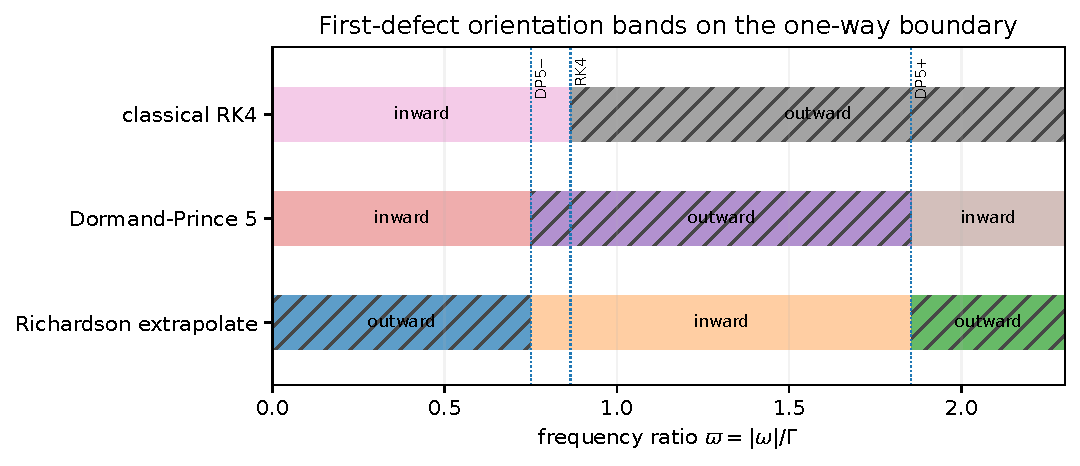
\includegraphics[width=0.90\textwidth]{FigS1_frequency_bands.pdf}
 \caption{Small-step orientation bands for classical RK4, Dormand--Prince 5, and the Richardson extrapolate of RK4. Dormand--Prince 5 and the extrapolate share the same frequency factor $G_6$ but have opposite first-defect signs, so their inward/outward bands are reversed.}
 \label{fig:supp_frequency_bands}
\end{figure}

\section{Complete laboratory-frame RK4 classification and conditioning}
For one-way, zero-dephasing RK4,
\begin{equation}
 M_4(x;\varpi)=-\frac{x^5q}{147456}\mathcal C_q(qx),\qquad
 \mathcal C_q(y)=y^3-16y^2-32(q-6)y+384(q-4).
\end{equation}
The discriminant is $16384(q-4)(8q^2-123q+348)$. With $q_\pm=(123\pm11\sqrt{33})/16$,
\begin{align}
\mathcal C_{q_-}(y)&=(y-9+\sqrt{33})^2(y-2\sqrt{33}+2),\\
\mathcal C_4(y)&=y(y-8)^2,\\
\mathcal C_{q_+}(y)&=(y-9-\sqrt{33})^2(y+2+2\sqrt{33}).
\end{align}
These factorizations and the population ceiling yield the six regimes stated in the article. The double root at $q_+$ produces square-root root separation and poor companion-matrix conditioning. On the tested binary64 platform, a companion-root implementation intermittently returned no eligible positive roots only four representable increments above $\varpi_+$. Exact Sturm isolation remains stable and is the scientific decision path.

For $q\to\infty$, $x_-=3/\varpi^2+O(\varpi^{-4})$ and $x_+=2\sqrt2/|\varpi|+O(\varpi^{-2})$. The isolated equality points at $q=4$ and $q=q_+$ are exact members of the mathematical CPTP set but are excluded as robust controller targets.

\section{Buffered and noncommuting persistence}
The five exact phase-covariant cases in the article have the following complete CPTP regions at $\varpi=2$:
\begin{center}
\begin{tabular}{lllll}
\toprule
$\theta$ & $\kappa$ & $r_1$ & $r_2$ & $r_3$\\
\midrule
$0$ & $10^{-3}$ & 0.253348869116 & 0.740695999652 & 1.269542711140\\
$10^{-3}$ & $0$ & 0.122268903470 & 0.742558312554 & 1.270544370136\\
$10^{-3}$ & $10^{-3}$ & 0.262033333161 & 0.738364627213 & 1.269753570826\\
$0$ & $10^{-2}$ & 0.519308218820 & 0.681621610068 & 1.262280154980\\
$10^{-2}$ & $0$ & 0.276930275811 & 0.720896805059 & 1.272391394935\\
\bottomrule
\end{tabular}
\end{center}
Each set is $[0,r_1]\cup[r_2,r_3]$. Exact numerator polynomials, root brackets, and sign samples are included in the machine-readable certificate.

For the transverse-field generator, column vectorization is used:
\begin{equation}
 \operatorname{vec}(AXB)=(B^T\otimes A)\operatorname{vec}(X).
\end{equation}
The full Liouvillian is
\begin{equation}
 L=-\ii(I\otimes H-H^T\otimes I)+\sum_k\gamma_k\left(\bar L_k\otimes L_k-\frac12I\otimes L_k^\dagger L_k-\frac12(L_k^\dagger L_k)^T\otimes I\right),
\end{equation}
with $H=-\omega\sigma_z/2+\Omega_x\sigma_x/2$. The RK4 superoperator is $S_4=I+hL+(hL)^2/2+(hL)^3/6+(hL)^4/24$. The Choi matrix is constructed as $J=\sum_{jk}E_{jk}\otimes\operatorname{unvec}(S_4\operatorname{vec}E_{jk})$. Every principal-minor numerator is an exact polynomial in $h$; all roots are isolated by Sturm sequences.

At $\theta=\kappa=10^{-3}$ and $\omega/\Gamma=2$, the following four parameter values are certified independently:
\begin{center}
\begin{tabular}{llll}
\toprule
$\Omega_x$ & attached upper & detached lower & detached upper\\
\midrule
0 & 0.262033333161 & 0.738364627213 & 1.269753570826\\
0.05 & 0.262418936401 & 0.737744306425 & 1.269432714005\\
0.10 & 0.263576909875 & 0.735883813007 & 1.268472478717\\
0.20 & 0.268222457925 & 0.728458223265 & 1.264665614699\\
\bottomrule
\end{tabular}
\end{center}
For $\Omega_x/\Gamma=0.1$, exact characteristic-polynomial brackets give smallest-Choi-eigenvalue signs $+,-,+,-$ at $h=0.1,0.5,0.9,1.4$, with approximate bracket midpoints $9.5156\times10^{-5}$, $-2.7778\times10^{-3}$, $5.8959\times10^{-4}$, and $-3.9227\times10^{-1}$. The four rows above are pointwise certificates; no uniform enclosure over $0\le\Omega_x/\Gamma\le0.2$ is claimed.

\section{Candidate maps, composition, and extrapolation}
For phase-covariant maps with the same stationary population,
\begin{equation}
 \Phi_\theta(a_2,c_2)\circ\Phi_\theta(a_1,c_1)=\Phi_\theta(a_2a_1,c_2c_1).
\end{equation}
The equal-$n$-substep candidate over total step $x$ therefore has
\begin{equation}
 a_n=R(-x/n)^n,\qquad c_n=R[-(x/2+u-\ii\nu)/n]^n.
\end{equation}
On the one-way nonnegative-population branch, the composite candidate is CPTP exactly when the substep is CPTP. Classical RK4 has $R_4(-x)>0$ for every $x\ge0$, so the total-step set of its equal-$n$-substep candidate is exactly $n\mathcal A_4$.

If a direct component is $\mathcal A=[x_-,x_+]$, consecutive substep-candidate sets overlap exactly when
\begin{equation}
 n x_+\ge(n+1)x_-
 \quad\Longleftrightarrow\quad
 \frac{x_+}{x_-}\ge\frac{n+1}{n}.
\end{equation}
The $n=1$ case is also the fixed-halving condition. The exact transition occurs at
\begin{equation}
 72q^3-2071q^2+12552q-21744=0,
 \qquad
 \varpi_{1/2}=2.248254604514980\ldots,
\end{equation}
where the relevant algebraic root lies in the detached RK4 regime. The resultant factorization is $6291456(q-4)(72q^3-2071q^2+12552q-21744)$; the two smaller cubic roots lie in the narrow reentrant band and do not define a detached component to skip.

At $\varpi=2$, exact isolation gives
\begin{align}
 \mathcal A_4&=\{0\}\cup[0.7447824278959\ldots,1.2703346269739\ldots],\\
 \mathcal A_4^{(2)}&=\{0\}\cup[1.4895648557918\ldots,2.5406692539478\ldots].
\end{align}
Their nontrivial positive-step components are disjoint; the full sets share only $x=0$. Thus $x=1$ is physical for the full candidate but not the two-half-step candidate, whereas $x=2$ reverses the two statuses. At this frequency every consecutive pair with $n\ge2$ overlaps, making the coarse/fine step-doubling pair the most restrictive pair in the equal-substep ladder.

For nonrotating one-way damping, define the coarse map $\Phi_{\rm c}$, the two-half-step map $\Phi_{\rm f}$, and the Richardson candidate
\begin{equation}
 \Phi_{\rm ext}=\frac{16\Phi_{\rm f}-\Phi_{\rm c}}{15}.
\end{equation}
This candidate has the stability function
\begin{equation}
 R_{\rm ext}(z)=\frac{16R_4(z/2)^2-R_4(z)}{15}
 =\sum_{j=0}^{5}\frac{z^j}{j!}+\frac{z^6}{864}+\frac{z^7}{8640}+\frac{z^8}{138240},
\end{equation}
so its first exponential defect is $\eta_6=-1/4320$. The general first-defect theorem gives
\begin{equation}
 M_{\rm ext}(x;\varpi)=-\frac{G_6(\varpi)}{4320}x^6+O(x^7),
 \qquad
 G_6=\frac{q(q^2-18q+48)}{32}.
\end{equation}
Hence the extrapolate is outward, inward, and outward as $\varpi$ crosses
\begin{equation}
 \sqrt{2-\sqrt{33}/4},\qquad \sqrt{2+\sqrt{33}/4}.
\end{equation}
Dormand--Prince 5 has the opposite sequence because its $\eta_6$ has the opposite sign; Fig.~\ref{fig:supp_frequency_bands} displays the comparison.

At $\varpi=0$, the Choi margin factors as
\begin{equation}
 M_{\rm ext}(x)=-\frac{x^6P_{10}(x)}{1252412463513600},
\end{equation}
where
\begin{align}
P_{10}(x)={}&x^{10}-64x^9+2304x^8-59392x^7+1183744x^6\\
&-19169280x^5+258932736x^4-2960916480x^3\\
&+19888865280x^2-97391738880x+280850595840.
\end{align}
The leading coefficient is $-31/138240$. A Sturm sequence places the first positive root of $P_{10}$ at $6.034523958649\ldots$, above the RK4 population ceiling $\alpha_4=2.785293563405\ldots$. Thus both constituents are CPTP for $0\le x\le\alpha_4$, while the extrapolated candidate is non-CPTP for every $0<x\le\alpha_4$. The first positive population-floor and margin roots are separated by only $1.40\times10^{-4}$, illustrating why visual sampling is inadequate. Globally, the extrapolate re-enters on
\begin{equation}
 [\rho_-,\rho_+]
 =[6.034523958649\ldots,6.459127767826\ldots],
\end{equation}
with the lower boundary set by the Choi margin and the upper boundary by the population ceiling.

\section{Executed-map certification and CP projection}
The guard has three outcomes: \textsc{pass}, \textsc{fail}, or \textsc{uncertain}. A binary64 input is interpreted through its exact IEEE-754 rational value, not through its printed decimal. The immutable candidate record contains the executed step, construction rule, numerical map, and certificate; the local-error observation is stored separately. Exact-exponential and exact-subflow maps receive a by-construction CPTP certificate only when built internally from a recognized construction rule; an arbitrary numerical matrix cannot receive one.

At $\varpi=2$, the printed decimal $1.270334626973889$ has a small positive margin, whereas the actual binary64 value represented by that display has a small negative margin. The former is therefore \textsc{pass} and the latter \textsc{fail}. Likewise, a legacy absolute tolerance $10^{-12}$ falsely accepts the negative margins at $x=0.004,10^{-3},10^{-4},10^{-5}$. These cases are regression tests.

For explicit phase-covariant polynomial candidates, exact constraint polynomials and Sturm isolation produce the admissible set below the current proposal within the certified domain. Roots are compared with both endpoints before their brackets are restricted: exterior roots are discarded, endpoint roots are retained, and interior roots are re-isolated. Equality points require joint certification of every active predicate. Any unresolved membership, identity, ordering, or sign yields \textsc{uncertain}.

Every positive-width component contains rational step specifications, but projection additionally requires a binary64 value whose exact rational lies in the component. The candidate is recertified at that value. Search or recertification failure yields \textsc{uncertain} with \texttt{EXECUTED\_BINARY\_RECERTIFICATION\_FAILED}; no admissible component yields \textsc{no component}.

A CP-only rejection does not update the PI error history. After projection, the actual candidate is reconstructed and its local error is recomputed. Error history is updated only from that new error value; a method or frame switch resets controller memory by policy.

\section{Adaptive tolerance sweep}
The channel-level step-doubling estimate is
\begin{equation}
 e(h)=\frac1{15}\,\frac12\left\|\frac{J[R_4(hL)]-J[R_4(hL/2)^2]}{2}\right\|_1.
\end{equation}
The fine specification $R_4(hL/2)^2$ defines the candidate to be executed. The benchmark uses a PI-type proposal with safety $0.9$, reconstructs and re-evaluates the candidate after every CP intervention, and compares error-only laboratory-frame RK4, a CP guard with rotating-frame fallback, rotating-frame RK4, and Strang splitting of exact subflows. The exact map $\exp(TL)$ is the reference. In the principal boundary sweep, every guarded acceptance uses rotating-frame fallback. Separate buffered and near-saddle runs exercise direct retention, locator invocation, and certified projection at global normalized-Choi errors below $10^{-3}$. The historical tolerance-$10$ projection case is retained only as an adversarial functionality test.

% Generated mechanically from results/v34/adaptive_benchmark_v34.csv. Do not edit by hand.
\begin{table*}[t]
\centering
\caption{Adaptive safety benchmark. The work proxy counts RK stage evaluations or exponential actions. Algebraic certification costs are excluded and reported separately in Table~\ref{tab:guard_telemetry}.}
\label{tab:adaptive_matrix}
\resizebox{0.99\textwidth}{!}{%
\begin{tabular}{llrrrrrr}
\toprule
Case & Policy & Choi error & Min. eig. & Direct & Projected & Fallback & RK stages\\
\midrule
boundary & error only & $7.92\times 10^{-4}$ & $-1\times 10^{-3}$ & 0 & 0 & 0 & 72\\
boundary & guard + rotating fallback & $7.45\times 10^{-6}$ & $\ge -10^{-15}$ & 0 & 0 & 4 & 132\\
boundary & rotating frame & $1.27\times 10^{-4}$ & $\ge -10^{-15}$ & 0 & 0 & 0 & 36\\
boundary & Strang & $8.33\times 10^{-17}$ & $\ge -10^{-15}$ & 0 & 0 & 0 & 0\\
buffered & guard, buffered & $2.85\times 10^{-4}$ & $\ge -10^{-15}$ & 3 & 2 & 0 & 84\\
buffered & guard, buffered/direct & $2.47\times 10^{-4}$ & $\ge -10^{-15}$ & 5 & 0 & 0 & 60\\
near saddle & guard, near saddle & $2.1\times 10^{-4}$ & $\ge -10^{-15}$ & 1 & 1 & 0 & 48\\
\bottomrule
\end{tabular}%
}
\end{table*}

\begin{table*}[t]
\centering
\caption{Guard telemetry. A locator call is counted on every invocation, including empty and uncertain outcomes. Root-isolation operations count exact Sturm-isolation calls; certification operations count candidate and component certifications, including binary recertification attempts.}
\label{tab:guard_telemetry}
\resizebox{0.99\textwidth}{!}{%
\begin{tabular}{lrrrrrrrrrr}
\toprule
Case & Tol. & Locator & Proj. found & Empty & Uncertain & Root iso. & Cert. & Binary & Prec. esc. & Fallback\\
\midrule
boundary & $1\times 10^{-2}$ & 3 & 0 & 3 & 0 & 9 & 21 & 0 & 0 & 3\\
boundary & $3\times 10^{-3}$ & 3 & 0 & 3 & 0 & 9 & 21 & 0 & 0 & 3\\
boundary & $1\times 10^{-3}$ & 4 & 0 & 4 & 0 & 12 & 33 & 0 & 0 & 4\\
boundary & $3\times 10^{-4}$ & 5 & 0 & 5 & 0 & 15 & 42 & 0 & 0 & 5\\
buffered & $1\times 10^{-3}$ & 2 & 2 & 0 & 0 & 6 & 25 & 2 & 0 & 0\\
buffered & $3\times 10^{-4}$ & 0 & 0 & 0 & 0 & 0 & 15 & 0 & 0 & 0\\
near saddle & $1\times 10^{-3}$ & 1 & 1 & 0 & 0 & 3 & 14 & 1 & 0 & 0\\
\bottomrule
\end{tabular}%
}
\end{table*}


The CSV and JSON records contain the candidate decisions and operation counts shown in Table~\ref{tab:guard_telemetry}. The work proxy counts only RK stages and exponential actions. Strang splitting is exact for this commuting decomposition and serves as a structural reference, not a universal timing comparison.

\section{Bell witness and fixed-horizon asymptotics}
For the one-way map, the normalized Bell output is $J/2$. If its active lower eigenvalue is negative, the total negative mass is $\delta_{\rm CP}=-\lambda_-/2$. The normalized-Choi trace error is
\begin{equation}
 E_\Omega=\frac12\left\|J_R/2-J_{\rm ex}/2\right\|_1.
\end{equation}
Trace preservation makes the difference traceless and gives $\delta_{\rm CP}\le E_\Omega$. At $x=10^{-2}$ the ratios for $\varpi=1,2,5$ are $0.341,0.909,0.441$.

For $N$ identical steps at $\theta=0$,
\begin{equation}
 M_N=(a-|c|^2)\sum_{j=0}^{N-1}a^{N-1-j}|c|^{2j}.
\end{equation}
If $a\ge0$, the repeated map is CPTP exactly when the one-step map is. On nonrotating damping, with $x_N=X/N$ and $K=(-1)^m(1-2^{1-m})\eta_m$,
\begin{align}
M_N(X)&=KX\e^{-X}(X/N)^{m-1}+O(N^{-m}),\\
p_{-,N}^{\rm RK}(X)&=\frac{KX\e^{-X}}{2(1+\e^{-X})}(X/N)^{m-1}+O(N^{-m}).
\end{align}
Negativity follows asymptotically only when $K<0$. Forward Euler and SSPRK(3,3) have exact negative one-step margins throughout the positive-population refinement range, which supplies the finite-$N$ sign used in the article.

\begin{figure}[t]
 \centering
 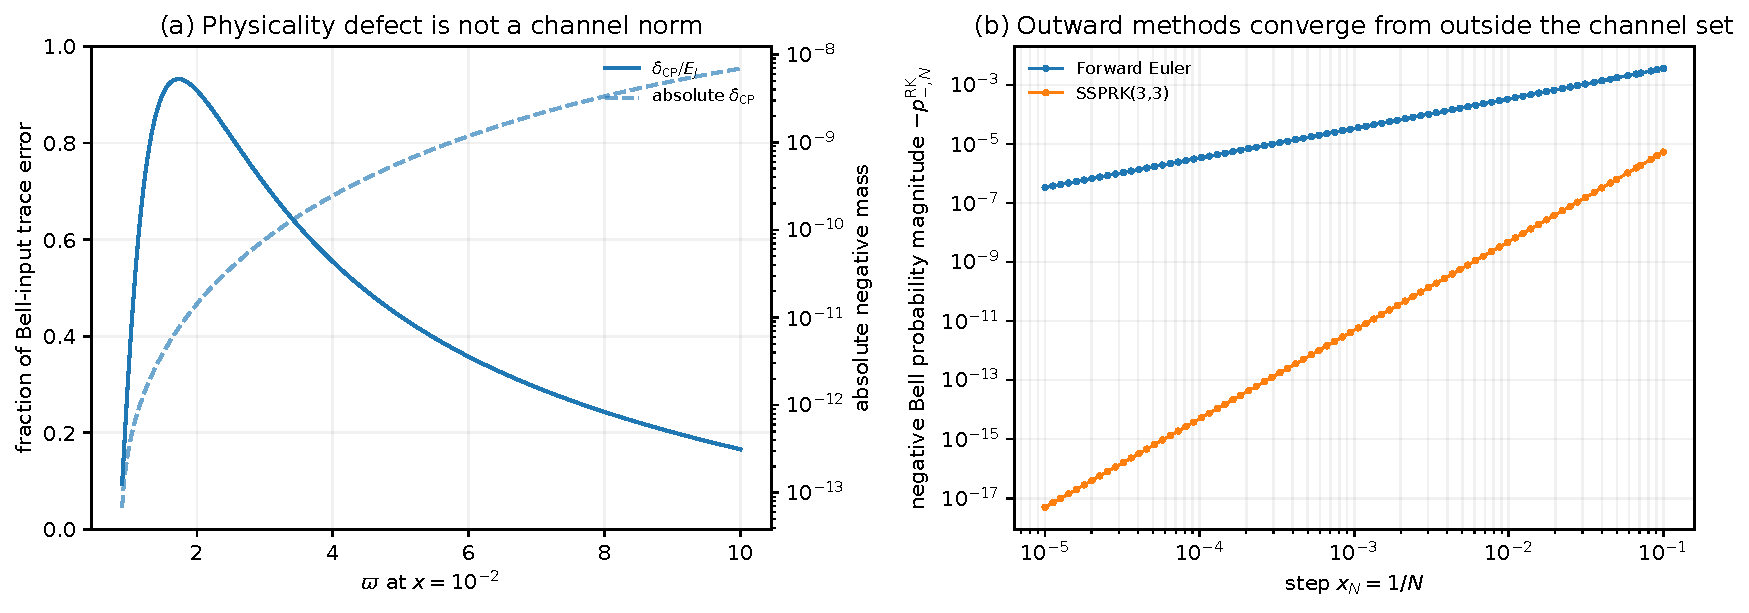
\includegraphics[width=0.90\textwidth]{FigS2_operational_refinement.pdf}
 \caption{Operational defect and fixed-horizon refinement. The negative normalized-Choi eigenvalue is a Bell-input positivity defect, not a worst-case channel norm. In the certified outward examples its sign remains negative while its magnitude decays at the predicted global order.}
 \label{fig:supp_operational}
\end{figure}

\section{Summary}
\begin{center}
\begin{tabularx}{\textwidth}{@{}X l l@{}}
\toprule
Method & Stage domain on $x\geq0$ & Certified admissible set \\
\midrule
Forward Euler & all $x\geq0$ & $\{0\}$ \\
Heun RK2 & all $x\geq0$ & $[0,2]$ \\
SSPRK(3,3) & all $x\geq0$ & $\{0\}$ \\
Classical RK4 & all $x\geq0$ & $[0,\alpha_4]$ \\
RK4 Richardson extrapolate & all $x\geq0$ & $\{0\}\cup[\rho_-,\rho_+]$ \\
Dormand-Prince 5 principal formula & all $x\geq0$ & $[0,\alpha_5]$ \\
Dormand-Prince embedded 4 formula & all $x\geq0$ & $\{0\}\cup[\beta_-,\beta_+]$ \\
Backward Euler & all $x\geq0$ & $[0,\infty)$ \\
Implicit midpoint & all $x\geq0$ & $\{0\}$ \\
\bottomrule
\end{tabularx}
\end{center}
\section{Forward Euler}
The exact stability function is
\[\begin{adjustbox}{max width=0.98\textwidth}$\displaystyle R(s)=s + 1$\end{adjustbox}\]
The full- and half-step stage-resolvent factors are $1$ and $1$, respectively.
The exact scalar functions are
\[\begin{adjustbox}{max width=0.98\textwidth}$\displaystyle a(x)=1 - x$\end{adjustbox}\]
\[\begin{adjustbox}{max width=0.98\textwidth}$\displaystyle M_R(x,0,0)=- \frac{x^{2}}{4}$\end{adjustbox}\]
The primitive boundary numerators below isolate the zeros of $a$, $a-1$, and $M_R$; their signs are retained in the exact expressions above and in every interval row.
\[\begin{aligned}
P_0(x)={}&x-1
\end{aligned}\]
\[\begin{aligned}
P_1(x)={}&x
\end{aligned}\]
\[\begin{aligned}
P_M(x)={}&x^{2}
\end{aligned}\]
These equations correspond respectively to $a(x)=0$, $a(x)=1$, and $M_R(x,0,0)=0$. Their square-free parts are
\[\begin{aligned}
\operatorname{sqf}P_0={}&x-1
\end{aligned}\]
\[\begin{aligned}
\operatorname{sqf}P_1={}&x
\end{aligned}\]
\[\begin{aligned}
\operatorname{sqf}P_M={}&x
\end{aligned}\]
\begin{center}
\begin{tabularx}{\textwidth}{@{}l l l X@{}}
\toprule
Label & Certified rational bracket & Approx. & Source / active mechanism \\
\midrule
$--$ & $1$ & $1$ & population floor (a=0) \\
\bottomrule
\end{tabularx}
\end{center}
\begin{center}
\begin{tabular}{@{}l c c c c c@{}}
\toprule
Open interval & $\operatorname{sgn}a$ & $\operatorname{sgn}(a-1)$ & $\operatorname{sgn}M$ & domain & CPTP \\
\midrule
$(0,1)$ & + & - & - & yes & no \\
$(1,\infty)$ & - & - & - & yes & no \\
\bottomrule
\end{tabular}
\end{center}
The certified admissible set is $\mathcal A_R=\{0\}$. The first exponential defect is $(m,\eta_m)=(2,- \frac{1}{2})$, and the signed boundary-law coefficient is $- \frac{1}{4}$.
\section{Heun RK2}
The exact stability function is
\[\begin{adjustbox}{max width=0.98\textwidth}$\displaystyle R(s)=\frac{s^{2}}{2} + s + 1$\end{adjustbox}\]
The full- and half-step stage-resolvent factors are $1$ and $1$, respectively.
The exact scalar functions are
\[\begin{adjustbox}{max width=0.98\textwidth}$\displaystyle a(x)=\frac{x^{2} - 2 x + 2}{2}$\end{adjustbox}\]
\[\begin{adjustbox}{max width=0.98\textwidth}$\displaystyle M_R(x,0,0)=- \frac{x^{3} \left(x - 8\right)}{64}$\end{adjustbox}\]
The primitive boundary numerators below isolate the zeros of $a$, $a-1$, and $M_R$; their signs are retained in the exact expressions above and in every interval row.
\[\begin{aligned}
P_0(x)={}&x^{2}-2 x+2
\end{aligned}\]
\[\begin{aligned}
P_1(x)={}&x^{2}-2 x
\end{aligned}\]
\[\begin{aligned}
P_M(x)={}&x^{4}-8 x^{3}
\end{aligned}\]
These equations correspond respectively to $a(x)=0$, $a(x)=1$, and $M_R(x,0,0)=0$. Their square-free parts are
\[\begin{aligned}
\operatorname{sqf}P_0={}&x^{2}-2 x+2
\end{aligned}\]
\[\begin{aligned}
\operatorname{sqf}P_1={}&x^{2}-2 x
\end{aligned}\]
\[\begin{aligned}
\operatorname{sqf}P_M={}&x^{2}-8 x
\end{aligned}\]
\begin{center}
\begin{tabularx}{\textwidth}{@{}l l l X@{}}
\toprule
Label & Certified rational bracket & Approx. & Source / active mechanism \\
\midrule
$--$ & $2$ & $2$ & population ceiling (a=1) \\
$--$ & $8$ & $8$ & coherence-population block (M=0) \\
\bottomrule
\end{tabularx}
\end{center}
\begin{center}
\begin{tabular}{@{}l c c c c c@{}}
\toprule
Open interval & $\operatorname{sgn}a$ & $\operatorname{sgn}(a-1)$ & $\operatorname{sgn}M$ & domain & CPTP \\
\midrule
$(0,2)$ & + & - & + & yes & yes \\
$(2,8)$ & + & + & + & yes & no \\
$(8,\infty)$ & + & + & - & yes & no \\
\bottomrule
\end{tabular}
\end{center}
The certified admissible set is $\mathcal A_R=[0,2]$. The first exponential defect is $(m,\eta_m)=(3,- \frac{1}{6})$, and the signed boundary-law coefficient is $\frac{1}{8}$.
\section{SSPRK(3,3)}
The exact stability function is
\[\begin{adjustbox}{max width=0.98\textwidth}$\displaystyle R(s)=\frac{s^{3}}{6} + \frac{s^{2}}{2} + s + 1$\end{adjustbox}\]
The full- and half-step stage-resolvent factors are $1$ and $1$, respectively.
The exact scalar functions are
\[\begin{adjustbox}{max width=0.98\textwidth}$\displaystyle a(x)=- \frac{x^{3} - 3 x^{2} + 6 x - 6}{6}$\end{adjustbox}\]
\[\begin{adjustbox}{max width=0.98\textwidth}$\displaystyle M_R(x,0,0)=- \frac{x^{4} \left(x^{2} - 12 x + 84\right)}{2304}$\end{adjustbox}\]
The primitive boundary numerators below isolate the zeros of $a$, $a-1$, and $M_R$; their signs are retained in the exact expressions above and in every interval row.
\[\begin{aligned}
P_0(x)={}&x^{3}-3 x^{2}+6 x\\
&-6
\end{aligned}\]
\[\begin{aligned}
P_1(x)={}&x^{3}-3 x^{2}+6 x
\end{aligned}\]
\[\begin{aligned}
P_M(x)={}&x^{6}-12 x^{5}+84 x^{4}
\end{aligned}\]
These equations correspond respectively to $a(x)=0$, $a(x)=1$, and $M_R(x,0,0)=0$. Their square-free parts are
\[\begin{aligned}
\operatorname{sqf}P_0={}&x^{3}-3 x^{2}+6 x\\
&-6
\end{aligned}\]
\[\begin{aligned}
\operatorname{sqf}P_1={}&x^{3}-3 x^{2}+6 x
\end{aligned}\]
\[\begin{aligned}
\operatorname{sqf}P_M={}&x^{3}-12 x^{2}+84 x
\end{aligned}\]
\begin{center}
\begin{tabularx}{\textwidth}{@{}l l l X@{}}
\toprule
Label & Certified rational bracket & Approx. & Source / active mechanism \\
\midrule
$--$ & $(1.596071637983321,1.596071637983322)$ & $1.596071637983322$ & population floor (a=0) \\
\bottomrule
\end{tabularx}
\end{center}
\begin{center}
\begin{tabular}{@{}l c c c c c@{}}
\toprule
Open interval & $\operatorname{sgn}a$ & $\operatorname{sgn}(a-1)$ & $\operatorname{sgn}M$ & domain & CPTP \\
\midrule
$(0,1.596071637983322)$ & + & - & - & yes & no \\
$(1.596071637983322,\infty)$ & - & - & - & yes & no \\
\bottomrule
\end{tabular}
\end{center}
The certified admissible set is $\mathcal A_R=\{0\}$. The first exponential defect is $(m,\eta_m)=(4,- \frac{1}{24})$, and the signed boundary-law coefficient is $- \frac{7}{192}$.
\section{Classical RK4}
The exact stability function is
\[\begin{adjustbox}{max width=0.98\textwidth}$\displaystyle R(s)=\frac{s^{4}}{24} + \frac{s^{3}}{6} + \frac{s^{2}}{2} + s + 1$\end{adjustbox}\]
The full- and half-step stage-resolvent factors are $1$ and $1$, respectively.
The exact scalar functions are
\[\begin{adjustbox}{max width=0.98\textwidth}$\displaystyle a(x)=\frac{x^{4} - 4 x^{3} + 12 x^{2} - 24 x + 24}{24}$\end{adjustbox}\]
\[\begin{adjustbox}{max width=0.98\textwidth}$\displaystyle M_R(x,0,0)=- \frac{x^{5} \left(x^{3} - 16 x^{2} + 160 x - 1152\right)}{147456}$\end{adjustbox}\]
The primitive boundary numerators below isolate the zeros of $a$, $a-1$, and $M_R$; their signs are retained in the exact expressions above and in every interval row.
\[\begin{aligned}
P_0(x)={}&x^{4}-4 x^{3}+12 x^{2}\\
&-24 x+24
\end{aligned}\]
\[\begin{aligned}
P_1(x)={}&x^{4}-4 x^{3}+12 x^{2}\\
&-24 x
\end{aligned}\]
\[\begin{aligned}
P_M(x)={}&x^{8}-16 x^{7}+160 x^{6}\\
&-1152 x^{5}
\end{aligned}\]
These equations correspond respectively to $a(x)=0$, $a(x)=1$, and $M_R(x,0,0)=0$. Their square-free parts are
\[\begin{aligned}
\operatorname{sqf}P_0={}&x^{4}-4 x^{3}+12 x^{2}\\
&-24 x+24
\end{aligned}\]
\[\begin{aligned}
\operatorname{sqf}P_1={}&x^{4}-4 x^{3}+12 x^{2}\\
&-24 x
\end{aligned}\]
\[\begin{aligned}
\operatorname{sqf}P_M={}&x^{4}-16 x^{3}+160 x^{2}\\
&-1152 x
\end{aligned}\]
\begin{center}
\begin{tabularx}{\textwidth}{@{}l l l X@{}}
\toprule
Label & Certified rational bracket & Approx. & Source / active mechanism \\
\midrule
$\alpha_4$ & $(2.785293563405281,2.785293563405282)$ & $2.785293563405282$ & population ceiling (a=1) \\
$\mu_4$ & $(10.982425466293273,10.982425466293274)$ & $10.982425466293273$ & coherence-population block (M=0) \\
\bottomrule
\end{tabularx}
\end{center}
\begin{center}
\begin{tabular}{@{}l c c c c c@{}}
\toprule
Open interval & $\operatorname{sgn}a$ & $\operatorname{sgn}(a-1)$ & $\operatorname{sgn}M$ & domain & CPTP \\
\midrule
$(0,2.785293563405282)$ & + & - & + & yes & yes \\
$(2.785293563405282,10.982425466293273)$ & + & + & + & yes & no \\
$(10.982425466293273,\infty)$ & + & + & - & yes & no \\
\bottomrule
\end{tabular}
\end{center}
The certified admissible set is $\mathcal A_R=[0,\alpha_4]$. The first exponential defect is $(m,\eta_m)=(5,- \frac{1}{120})$, and the signed boundary-law coefficient is $\frac{1}{128}$.
\section{Dormand-Prince 5 principal formula}
The exact stability function is
\[\begin{adjustbox}{max width=0.98\textwidth}$\displaystyle R(s)=\frac{s^{6}}{600} + \frac{s^{5}}{120} + \frac{s^{4}}{24} + \frac{s^{3}}{6} + \frac{s^{2}}{2} + s + 1$\end{adjustbox}\]
The full- and half-step stage-resolvent factors are $1$ and $1$, respectively.
The exact scalar functions are
\[\begin{adjustbox}{max width=0.98\textwidth}$\displaystyle a(x)=\frac{x^{6} - 5 x^{5} + 25 x^{4} - 100 x^{3} + 300 x^{2} - 600 x + 600}{600}$\end{adjustbox}\]
\[\begin{adjustbox}{max width=0.98\textwidth}$\displaystyle M_R(x,0,0)=- \frac{x^{6} \left(x^{6} - 20 x^{5} + 300 x^{4} - 3600 x^{3} + 35600 x^{2} - 294400 x - 396800\right)}{1474560000}$\end{adjustbox}\]
The primitive boundary numerators below isolate the zeros of $a$, $a-1$, and $M_R$; their signs are retained in the exact expressions above and in every interval row.
\[\begin{aligned}
P_0(x)={}&x^{6}-5 x^{5}+25 x^{4}\\
&-100 x^{3}+300 x^{2}-600 x\\
&+600
\end{aligned}\]
\[\begin{aligned}
P_1(x)={}&x^{6}-5 x^{5}+25 x^{4}\\
&-100 x^{3}+300 x^{2}-600 x
\end{aligned}\]
\[\begin{aligned}
P_M(x)={}&x^{12}-20 x^{11}+300 x^{10}\\
&-3600 x^{9}+35600 x^{8}-294400 x^{7}\\
&-396800 x^{6}
\end{aligned}\]
These equations correspond respectively to $a(x)=0$, $a(x)=1$, and $M_R(x,0,0)=0$. Their square-free parts are
\[\begin{aligned}
\operatorname{sqf}P_0={}&x^{6}-5 x^{5}+25 x^{4}\\
&-100 x^{3}+300 x^{2}-600 x\\
&+600
\end{aligned}\]
\[\begin{aligned}
\operatorname{sqf}P_1={}&x^{6}-5 x^{5}+25 x^{4}\\
&-100 x^{3}+300 x^{2}-600 x
\end{aligned}\]
\[\begin{aligned}
\operatorname{sqf}P_M={}&x^{7}-20 x^{6}+300 x^{5}\\
&-3600 x^{4}+35600 x^{3}-294400 x^{2}\\
&-396800 x
\end{aligned}\]
\begin{center}
\begin{tabularx}{\textwidth}{@{}l l l X@{}}
\toprule
Label & Certified rational bracket & Approx. & Source / active mechanism \\
\midrule
$\alpha_5$ & $(3.306567892634946,3.306567892634947)$ & $3.306567892634947$ & population ceiling (a=1) \\
$\mu_5$ & $(13.174093462800933,13.174093462800934)$ & $13.174093462800933$ & coherence-population block (M=0) \\
\bottomrule
\end{tabularx}
\end{center}
\begin{center}
\begin{tabular}{@{}l c c c c c@{}}
\toprule
Open interval & $\operatorname{sgn}a$ & $\operatorname{sgn}(a-1)$ & $\operatorname{sgn}M$ & domain & CPTP \\
\midrule
$(0,3.306567892634947)$ & + & - & + & yes & yes \\
$(3.306567892634947,13.174093462800933)$ & + & + & + & yes & no \\
$(13.174093462800933,\infty)$ & + & + & - & yes & no \\
\bottomrule
\end{tabular}
\end{center}
The certified admissible set is $\mathcal A_R=[0,\alpha_5]$. The first exponential defect is $(m,\eta_m)=(6,\frac{1}{3600})$, and the signed boundary-law coefficient is $\frac{31}{115200}$.
\section{Dormand-Prince embedded 4 formula}
The exact stability function is
\[\begin{adjustbox}{max width=0.98\textwidth}$\displaystyle R(s)=\frac{s^{7}}{24000} + \frac{161 s^{6}}{120000} + \frac{1097 s^{5}}{120000} + \frac{s^{4}}{24} + \frac{s^{3}}{6} + \frac{s^{2}}{2} + s + 1$\end{adjustbox}\]
The full- and half-step stage-resolvent factors are $1$ and $1$, respectively.
The exact scalar functions are
\[\begin{adjustbox}{max width=0.98\textwidth}$\displaystyle a(x)=- \frac{5 x^{7} - 161 x^{6} + 1097 x^{5} - 5000 x^{4} + 20000 x^{3} - 60000 x^{2} + 120000 x - 120000}{120000}$\end{adjustbox}\]
\[\begin{adjustbox}{max width=0.98\textwidth}$\displaystyle M_R(x,0,0)=- \frac{x^{5} \left(25 x^{9} - 3220 x^{8} + 147564 x^{7} - 3225872 x^{6} + 48214544 x^{5} - 576320000 x^{4} + 5721600000 x^{3} - 37719040000 x^{2} + 16752640000 x + 178790400000\right)}{235929600000000}$\end{adjustbox}\]
The primitive boundary numerators below isolate the zeros of $a$, $a-1$, and $M_R$; their signs are retained in the exact expressions above and in every interval row.
\[\begin{aligned}
P_0(x)={}&5 x^{7}-161 x^{6}+1097 x^{5}\\
&-5000 x^{4}+20000 x^{3}-60000 x^{2}\\
&+120000 x-120000
\end{aligned}\]
\[\begin{aligned}
P_1(x)={}&5 x^{7}-161 x^{6}+1097 x^{5}\\
&-5000 x^{4}+20000 x^{3}-60000 x^{2}\\
&+120000 x
\end{aligned}\]
\[\begin{aligned}
P_M(x)={}&25 x^{14}-3220 x^{13}+147564 x^{12}\\
&-3225872 x^{11}+48214544 x^{10}-576320000 x^{9}\\
&+5721600000 x^{8}-37719040000 x^{7}+16752640000 x^{6}\\
&+178790400000 x^{5}
\end{aligned}\]
These equations correspond respectively to $a(x)=0$, $a(x)=1$, and $M_R(x,0,0)=0$. Their square-free parts are
\[\begin{aligned}
\operatorname{sqf}P_0={}&5 x^{7}-161 x^{6}+1097 x^{5}\\
&-5000 x^{4}+20000 x^{3}-60000 x^{2}\\
&+120000 x-120000
\end{aligned}\]
\[\begin{aligned}
\operatorname{sqf}P_1={}&5 x^{7}-161 x^{6}+1097 x^{5}\\
&-5000 x^{4}+20000 x^{3}-60000 x^{2}\\
&+120000 x
\end{aligned}\]
\[\begin{aligned}
\operatorname{sqf}P_M={}&25 x^{10}-3220 x^{9}+147564 x^{8}\\
&-3225872 x^{7}+48214544 x^{6}-576320000 x^{5}\\
&+5721600000 x^{4}-37719040000 x^{3}+16752640000 x^{2}\\
&+178790400000 x
\end{aligned}\]
\begin{center}
\begin{tabularx}{\textwidth}{@{}l l l X@{}}
\toprule
Label & Certified rational bracket & Approx. & Source / active mechanism \\
\midrule
$\beta_-$ & $(3.06885654805038,3.068856548050381)$ & $3.068856548050381$ & coherence-population block (M=0) \\
$\beta_+$ & $(4.384986320801944,4.384986320801945)$ & $4.384986320801944$ & population ceiling (a=1) \\
$\delta_M$ & $(15.298767807585426,15.298767807585427)$ & $15.298767807585427$ & coherence-population block (M=0) \\
$\delta_1$ & $(24.72775431876031,24.727754318760311)$ & $24.72775431876031$ & population ceiling (a=1) \\
$\delta_0$ & $(24.727895030129697,24.727895030129698)$ & $24.727895030129697$ & population floor (a=0) \\
\bottomrule
\end{tabularx}
\end{center}
\begin{center}
\begin{tabular}{@{}l c c c c c@{}}
\toprule
Open interval & $\operatorname{sgn}a$ & $\operatorname{sgn}(a-1)$ & $\operatorname{sgn}M$ & domain & CPTP \\
\midrule
$(0,3.068856548050381)$ & + & - & - & yes & no \\
$(3.068856548050381,4.384986320801944)$ & + & - & + & yes & yes \\
$(4.384986320801944,15.298767807585427)$ & + & + & + & yes & no \\
$(15.298767807585427,24.72775431876031)$ & + & + & - & yes & no \\
$(24.72775431876031,24.727895030129697)$ & + & - & - & yes & no \\
$(24.727895030129697,\infty)$ & - & - & - & yes & no \\
\bottomrule
\end{tabular}
\end{center}
The certified admissible set is $\mathcal A_R=\{0\}\cup[\beta_-,\beta_+]$. The first exponential defect is $(m,\eta_m)=(5,\frac{97}{120000})$, and the signed boundary-law coefficient is $- \frac{97}{128000}$.
\section{Backward Euler}
The exact stability function is
\[\begin{adjustbox}{max width=0.98\textwidth}$\displaystyle R(s)=- \frac{1}{s - 1}$\end{adjustbox}\]
The full- and half-step stage-resolvent factors are $x + 1$ and $\frac{x}{2} + 1$, respectively.
The exact scalar functions are
\[\begin{adjustbox}{max width=0.98\textwidth}$\displaystyle a(x)=\frac{1}{x + 1}$\end{adjustbox}\]
\[\begin{adjustbox}{max width=0.98\textwidth}$\displaystyle M_R(x,0,0)=\frac{x^{2}}{\left(x + 1\right) \left(x + 2\right)^{2}}$\end{adjustbox}\]
The primitive boundary numerators below isolate the zeros of $a$, $a-1$, and $M_R$; their signs are retained in the exact expressions above and in every interval row.
\[\begin{aligned}
P_0(x)={}&1
\end{aligned}\]
\[\begin{aligned}
P_1(x)={}&x
\end{aligned}\]
\[\begin{aligned}
P_M(x)={}&x^{2}
\end{aligned}\]
These equations correspond respectively to $a(x)=0$, $a(x)=1$, and $M_R(x,0,0)=0$. Their square-free parts are
\[\begin{aligned}
\operatorname{sqf}P_0={}&1
\end{aligned}\]
\[\begin{aligned}
\operatorname{sqf}P_1={}&x
\end{aligned}\]
\[\begin{aligned}
\operatorname{sqf}P_M={}&x
\end{aligned}\]
No positive real boundary roots or stage-resolvent singularities occur.
\begin{center}
\begin{tabular}{@{}l c c c c c@{}}
\toprule
Open interval & $\operatorname{sgn}a$ & $\operatorname{sgn}(a-1)$ & $\operatorname{sgn}M$ & domain & CPTP \\
\midrule
$(0,\infty)$ & + & - & + & yes & yes \\
\bottomrule
\end{tabular}
\end{center}
The certified admissible set is $\mathcal A_R=[0,\infty)$. The first exponential defect is $(m,\eta_m)=(2,\frac{1}{2})$, and the signed boundary-law coefficient is $\frac{1}{4}$.
\section{Implicit midpoint}
The exact stability function is
\[\begin{adjustbox}{max width=0.98\textwidth}$\displaystyle R(s)=- \frac{s + 2}{s - 2}$\end{adjustbox}\]
The full- and half-step stage-resolvent factors are $\frac{x}{2} + 1$ and $\frac{x}{4} + 1$, respectively.
The exact scalar functions are
\[\begin{adjustbox}{max width=0.98\textwidth}$\displaystyle a(x)=- \frac{x - 2}{x + 2}$\end{adjustbox}\]
\[\begin{adjustbox}{max width=0.98\textwidth}$\displaystyle M_R(x,0,0)=- \frac{2 x^{3}}{\left(x + 2\right) \left(x + 4\right)^{2}}$\end{adjustbox}\]
The primitive boundary numerators below isolate the zeros of $a$, $a-1$, and $M_R$; their signs are retained in the exact expressions above and in every interval row.
\[\begin{aligned}
P_0(x)={}&x-2
\end{aligned}\]
\[\begin{aligned}
P_1(x)={}&x
\end{aligned}\]
\[\begin{aligned}
P_M(x)={}&x^{3}
\end{aligned}\]
These equations correspond respectively to $a(x)=0$, $a(x)=1$, and $M_R(x,0,0)=0$. Their square-free parts are
\[\begin{aligned}
\operatorname{sqf}P_0={}&x-2
\end{aligned}\]
\[\begin{aligned}
\operatorname{sqf}P_1={}&x
\end{aligned}\]
\[\begin{aligned}
\operatorname{sqf}P_M={}&x
\end{aligned}\]
\begin{center}
\begin{tabularx}{\textwidth}{@{}l l l X@{}}
\toprule
Label & Certified rational bracket & Approx. & Source / active mechanism \\
\midrule
$--$ & $2$ & $2$ & population floor (a=0) \\
\bottomrule
\end{tabularx}
\end{center}
\begin{center}
\begin{tabular}{@{}l c c c c c@{}}
\toprule
Open interval & $\operatorname{sgn}a$ & $\operatorname{sgn}(a-1)$ & $\operatorname{sgn}M$ & domain & CPTP \\
\midrule
$(0,2)$ & + & - & - & yes & no \\
$(2,\infty)$ & - & - & - & yes & no \\
\bottomrule
\end{tabular}
\end{center}
The certified admissible set is $\mathcal A_R=\{0\}$. The first exponential defect is $(m,\eta_m)=(3,\frac{1}{12})$, and the signed boundary-law coefficient is $- \frac{1}{16}$.
\section{Embedded Dormand--Prince no-omission check}
For the embedded fourth-order formula, the ordered positive events are the first margin zero $\beta_-$, the first population-ceiling zero $\beta_+$, the second margin zero $\delta_M$, the second population-ceiling zero $\delta_1$, and the population-floor zero $\delta_0$. The complete sign chart shows that both CPTP inequalities hold only between $\beta_-$ and $\beta_+$. Population overflow excludes the region after $\beta_+$, the margin is again negative after $\delta_M$, and the population multiplier becomes negative after $\delta_0$. Consequently no later root generates an omitted admissible component.
\section{Reproducibility}
The companion machine-readable records contain exact expressions, rational brackets, root multiplicities, exact rational sample points, and interval truth values. The eight named RK formulas are generated directly from the exact tableaux in \texttt{src/rk\_choi\_margin/methods.py}; the Richardson stability polynomial and its global certificate are regenerated independently by \texttt{scripts/verify\_v33\_extensions.py}. Every displayed endpoint is produced by or checked against exact real-root isolation rather than visual sampling.


\end{document}
